% =============================================================================
% Apresentação (máx. 5 min) — ECM514 Projeto Desafio
% Compilação:  cd docs/apresentacao && make     (gera build/slides.pdf)
% Roteiro de fala: roteiro.md (mesma pasta), só local — fora do Git.
% Figuras lidas de results/figures/ e docs/relatorio/assets/, sem cópia.
% Todos os números vêm de results/metrics/ (os mesmos do relatório).
% =============================================================================
\documentclass[aspectratio=169,11pt]{beamer}

\usepackage[T1]{fontenc}
\usepackage[utf8]{inputenc}
\usepackage[brazil]{babel}
\usepackage{lmodern}
\usepackage{booktabs}
\usepackage{siunitx}
\sisetup{output-decimal-marker = {,}}
\DeclareSIUnit{\hp}{HP}

\graphicspath{{../../results/figures/}{../relatorio/assets/}}

% ---- Visual sóbrio: tema padrão, sem navegação, cores contidas ---------------
\usetheme{default}
\setbeamertemplate{navigation symbols}{}
\definecolor{azul}{HTML}{1C5CAB}
\definecolor{laranja}{HTML}{C2410C}
\definecolor{cinza}{HTML}{5F5E5A}
\setbeamercolor{frametitle}{fg=azul}
\setbeamercolor{title}{fg=azul}
\setbeamercolor{structure}{fg=azul}
\setbeamerfont{frametitle}{series=\bfseries,size=\Large}
\setbeamertemplate{itemize item}{\color{azul}$\blacktriangleright$}
\setbeamertemplate{footline}{%
  \hfill{\color{cinza}\scriptsize\insertframenumber/\inserttotalframenumber}\hspace{1em}\vspace{0.6em}}

\newcommand{\destaque}[1]{{\color{laranja}\bfseries #1}}
\newcommand{\nota}[1]{{\color{cinza}\footnotesize #1}}

\title{Detecção e diagnóstico de defeitos em rolamentos}
\subtitle{Alta acurácia no CWRU é fácil --- e diz pouco}
\author{André Maiolini \and Durval Santos \and Leonardo Amadio \\ Lucas Carvalho \and Estevan Feher}
\institute{ECM514 --- Ciência de Dados \\ Instituto Mauá de Tecnologia}
\date{2026}

\begin{document}

% ---------------------------------------------------------------- 1 (André)
\begin{frame}[plain]
  \titlepage
\end{frame}

% ---------------------------------------------------------------- 2 (André)
\begin{frame}{O problema e os dados}
  \begin{center}
    \emph{``Detectar que algo mudou é um problema; identificar o que mudou é outro, mais difícil.''}\\
    \nota{--- enunciado do projeto}
  \end{center}
  \vspace{-0.4em}
  \begin{columns}[T]
    \begin{column}{0.52\textwidth}
      \begin{itemize}
        \item \textbf{Detecção}: o comportamento mudou?\\
        \nota{treino só com sinais normais}
        \item \textbf{Diagnóstico}: qual é o defeito?\\
        \nota{normal, pista interna, pista externa, esfera}
        \item Dados: \textbf{CWRU}, acelerômetro do lado do acionamento, \SI{12}{\kilo\hertz}
        \item Protocolo: treino em 0--\SI{2}{\hp}, teste em \SI{3}{\hp}\\
        \nota{nunca dividir janelas da mesma gravação}
      \end{itemize}
    \end{column}
    \begin{column}{0.45\textwidth}
      \centering
      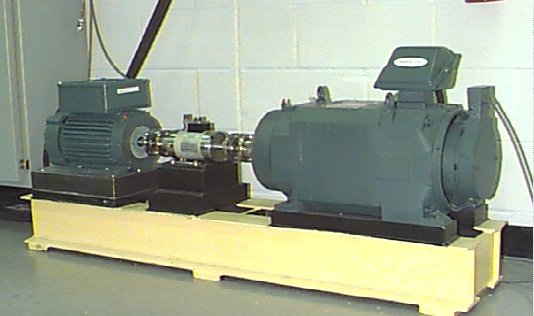
\includegraphics[width=0.85\linewidth]{CWRU_teststand.jpeg}\\
      \nota{Bancada do CWRU (Case Western Reserve University)}
    \end{column}
  \end{columns}
\end{frame}

% ---------------------------------------------------------------- 3 (Durval)
\begin{frame}{Antes de modelar: limpar os dados}
  \begin{columns}[T]
    \begin{column}{0.49\textwidth}
      \begin{itemize}
        \item Os normais estão a \destaque{\SI{48}{\kilo\hertz}}, não a 12
        \item \textbf{Decimação} por 4 com filtro anti-\emph{aliasing}
      \end{itemize}
    \end{column}
    \begin{column}{0.49\textwidth}
      \begin{itemize}
        \item Resíduo em 4,8--\SI{6}{\kilo\hertz} $\Rightarrow$ \textbf{mesma banda} para todos
        \item Janela: 4096 amostras $=$ 3 períodos da gaiola
      \end{itemize}
    \end{column}
  \end{columns}
  \vspace{0.3em}
  \centering
  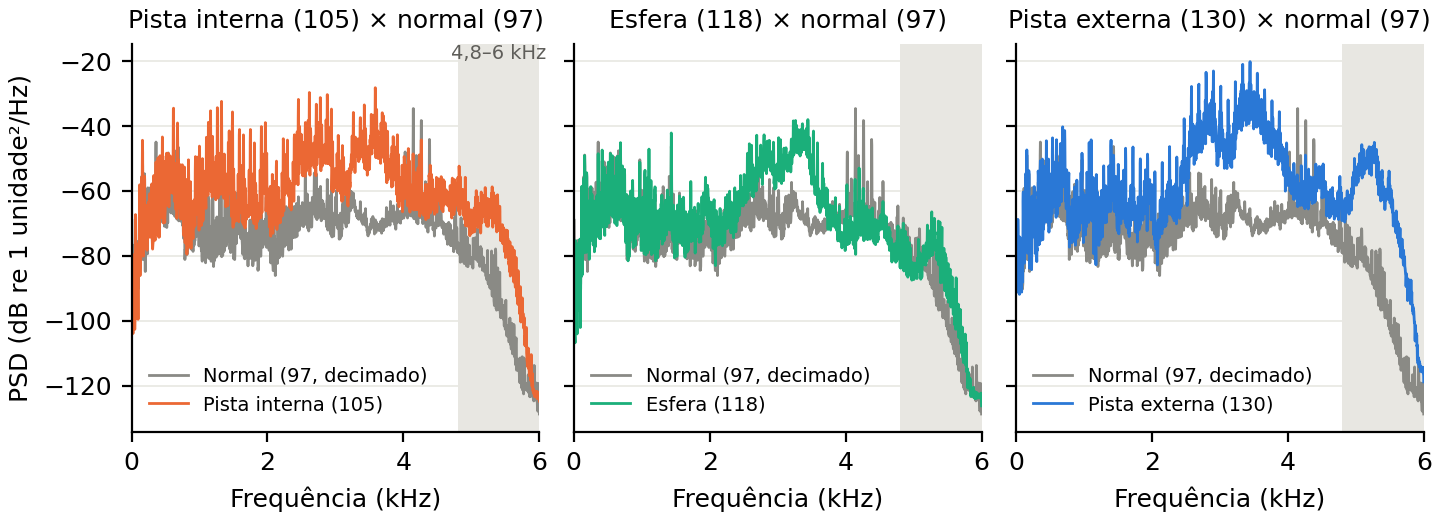
\includegraphics[width=0.9\textwidth]{espectro_normal_decimado_vs_falhas.png}\\
  \nota{Sem isso, o modelo separaria normal de falha pela taxa de amostragem.}
\end{frame}

% ---------------------------------------------------------------- 4 (Durval)
\begin{frame}{A física do defeito: o envelope}
  \begin{columns}[T]
    \begin{column}{0.40\textwidth}
      \begin{itemize}
        \item Cada defeito bate numa \textbf{frequência própria}, dada pela geometria e pela rotação:\\
        \nota{BPFO (pista externa), BPFI (interna), BSF (esfera)}
        \item O \textbf{espectro do envelope} mostra essa repetição
        \item Features: 5 do tempo (RMS, curtose\dots) + 3 \emph{scores} de envelope
      \end{itemize}
    \end{column}
    \begin{column}{0.58\textwidth}
      \centering
      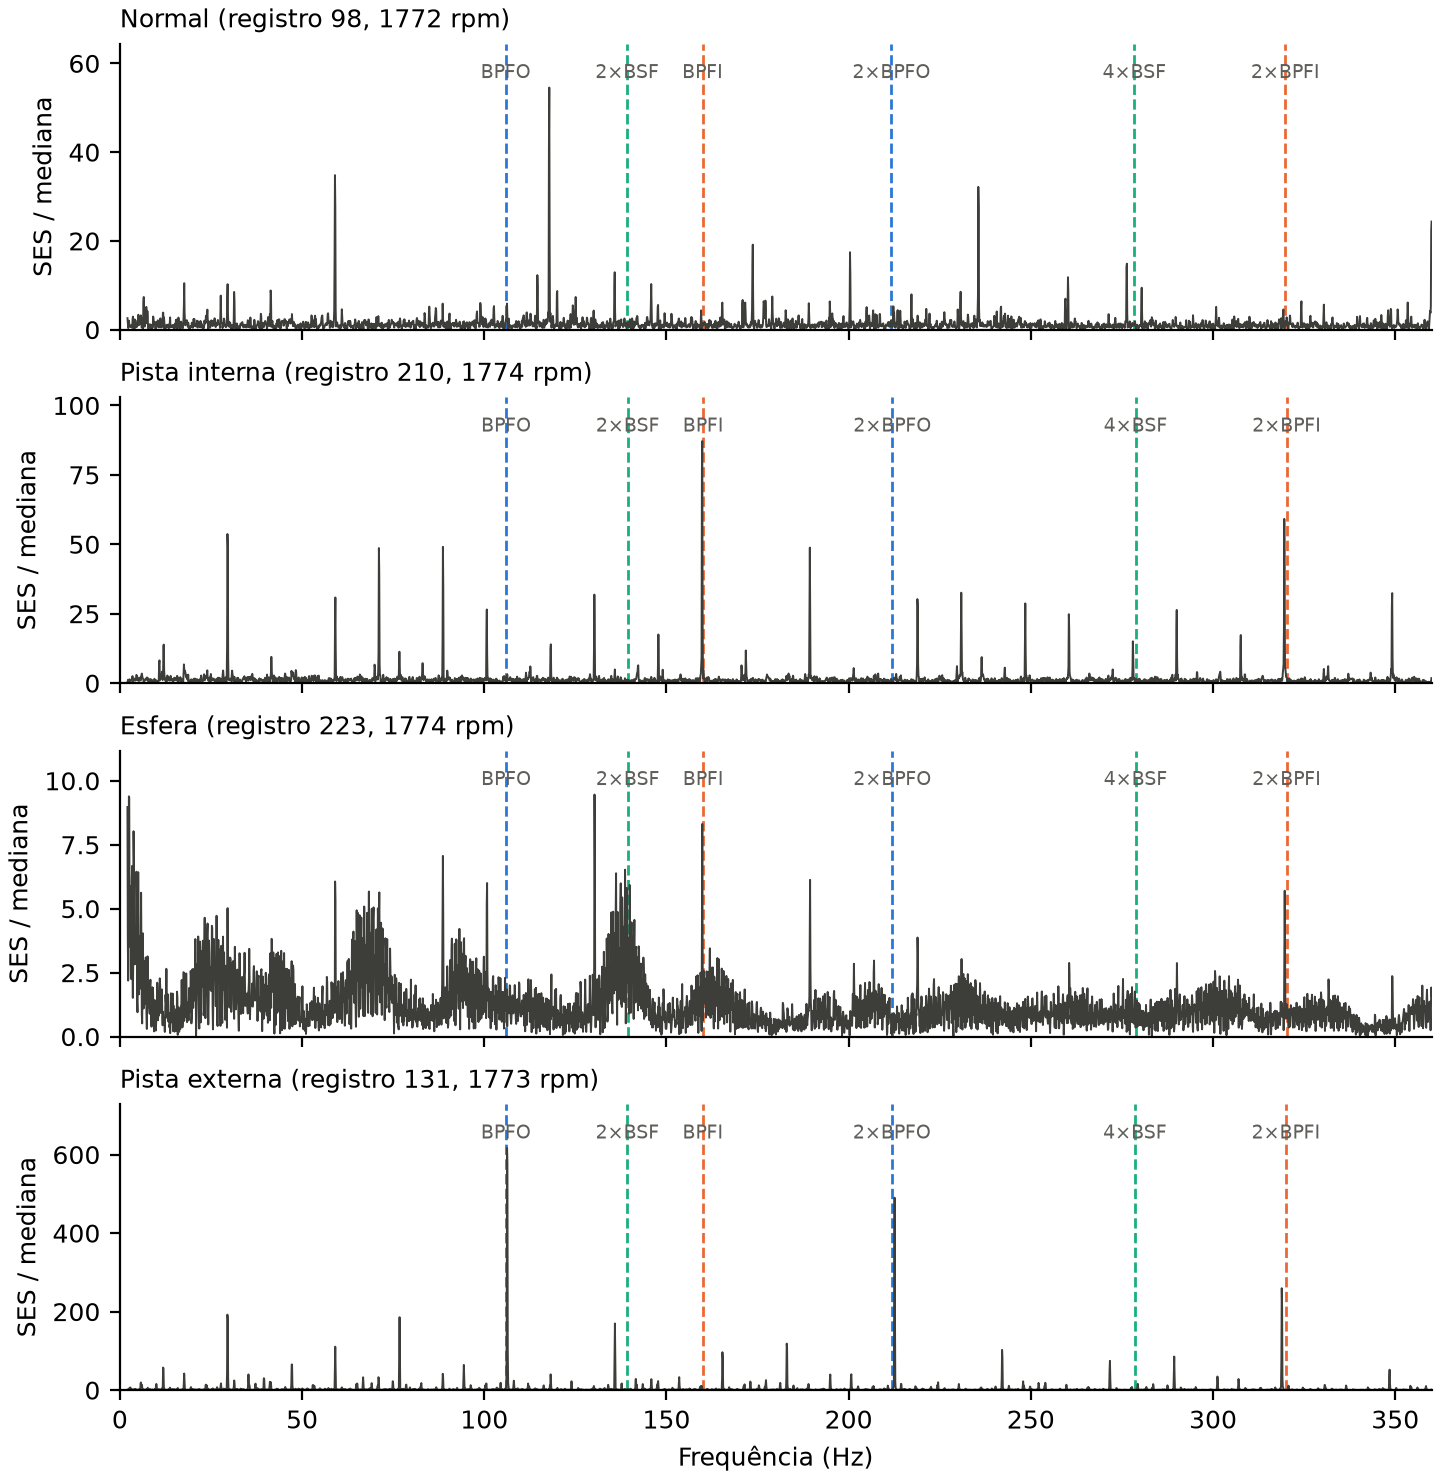
\includegraphics[height=0.78\textheight]{envelope_por_classe_1hp.png}
    \end{column}
  \end{columns}
\end{frame}

% ---------------------------------------------------------------- 5 (Leonardo)
\begin{frame}{Validação física: o pico cai onde a teoria prevê?}
  \centering
  \begin{tabular}{lccc}
    \toprule
    \textbf{Classe} & \textbf{Gravações} & \textbf{Confirmadas} & \textbf{Smith \& Randall (2015)} \\
    \midrule
    Pista interna            & 12 & \textbf{12} & 11 \\
    Pista externa (6 h)      & 12 & \textbf{8}  & 8 \\
    Pista externa (3 h/12 h) & 16 & \textbf{16} & 16 \\
    Esfera                   & 12 & \destaque{0} & 1 \\
    \bottomrule
  \end{tabular}

  \vspace{1.2em}
  \begin{itemize}
    \item Concorda com a auditoria de referência em \textbf{50 de 52} gravações
    \item Sem modelo nenhum: só geometria do rolamento + espectro do envelope
    \item \destaque{Na esfera, o defeito não aparece} no envelope
  \end{itemize}
\end{frame}

% ---------------------------------------------------------------- 6 (Leonardo)
\begin{frame}{Detecção: AUC = 1,00 \dots\ desconfie}
  \begin{columns}[T]
    \begin{column}{0.49\textwidth}
      \begin{itemize}
        \item 4 detectores treinados \textbf{só com normais}: AUC \textbf{1,00}
        \item Não é vazamento: o \destaque{RMS sozinho} dá AUC 1,00
      \end{itemize}
    \end{column}
    \begin{column}{0.49\textwidth}
      \begin{itemize}
        \item Falhas \emph{sem} defeito visível (200, 225): alarme em 100\%
        \item Precisão 0,99? 90\% do teste é falha:\\ \destaque{alarmar sempre} já dá 0,90
      \end{itemize}
    \end{column}
  \end{columns}
  \vspace{0.3em}
  \centering
  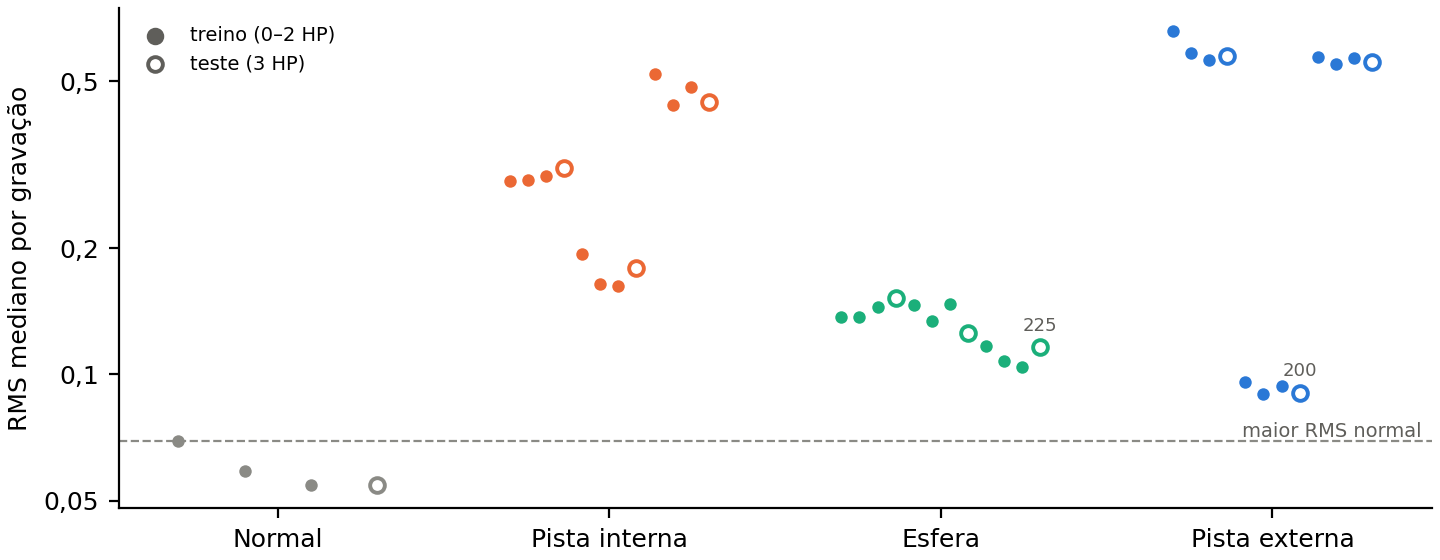
\includegraphics[width=0.85\textwidth]{rms_por_gravacao.png}\\
  \nota{Toda gravação de falha vibra mais que toda gravação normal.}
\end{frame}

% ---------------------------------------------------------------- 7 (Lucas)
\begin{frame}{Classificação: o roteiro das aulas}
  \begin{itemize}
    \item \texttt{Pipeline}(\texttt{StandardScaler}, modelo) $\rightarrow$ seleção por validação cruzada
    \item Validação \textbf{agrupada por carga} (\texttt{LeaveOneGroupOut}), não embaralhada
    \item 5 candidatos $\rightarrow$ Random Forest $\rightarrow$ \texttt{GridSearchCV}
  \end{itemize}
  \vspace{0.6em}
  \centering
  \begin{tabular}{lcc}
    \toprule
    & \textbf{Random Forest} & \textbf{CNN 1D} \\
    \midrule
    Acurácia no teste (\SI{3}{\hp})   & \textbf{95,7\%} & \textbf{99,7\%} \\
    Esfera: precisão / recall         & 0,88 / 0,99 & 0,99 / 1,00 \\
    Defeito em outra posição          & \destaque{40\%} & \destaque{64\%} \\
    \quad média entre sementes        & 48\% & 55\% \\
    \bottomrule
  \end{tabular}

  \vspace{0.6em}
  \nota{Esfera vira ``classe-refúgio'' (recall alto, precisão baixa). RMS + pico = 56\% da importância; \emph{score} da esfera, 3\%.}
\end{frame}

% ---------------------------------------------------------------- 8 (Estevan)
\begin{frame}{O teste decisivo: uma montagem nunca vista}
  \begin{itemize}
    \item No CWRU, cada defeito foi ensaiado numa \textbf{única montagem}, repetida nas 4 cargas
    \item Treinar em 2 diâmetros e testar no 3.º $=$ montagem nova \nota{(acaso: 33\%)}
  \end{itemize}
  \vspace{0.5em}
  \centering
  \begin{tabular}{lcc}
    \toprule
    & \textbf{Teste por carga} & \textbf{Montagem nova} \\
    \midrule
    Random Forest (tempo+envelope) & 95,7\% & \destaque{45,7\%} \\
    CNN 1D                         & 99,7\% & \destaque{49,8\%} \\
    \midrule
    \textbf{Regra física, sem treino} & --- & \textbf{65,7\%} \\
    \bottomrule
  \end{tabular}

  \vspace{0.6em}
  \nota{Só a regra física acerta mais montagens que o acaso (6 de 9, $p = 0{,}042$). Ela reconhece 99,8\% da pista externa em outra posição.}
\end{frame}

% ---------------------------------------------------------------- 9 (Estevan)
\begin{frame}{Conclusões}
  \begin{itemize}
    \item \textbf{Detectar} foi fácil demais (amplitude); \textbf{diagnosticar} não sobrevive a uma montagem nova
    \item No CWRU, \textbf{alta acurácia é fácil e diz pouco}: os modelos aprendem amplitude e montagem
    \item A \textbf{física generaliza} onde o aprendizado não generaliza
    \item O que funcionou: protocolo sem vazamento, ablações, validação física
    \item Limites: 4 gravações normais, defeitos artificiais, uma bancada
  \end{itemize}
  \vspace{1em}
  \centering
  \nota{Código, notebook (Colab) e relatório: \texttt{github.com/Nyfeu/Vibration\_Analysis}}
\end{frame}

\end{document}
